\documentclass[a4paper,12pt,oneside]{report}
\usepackage{graphicx}
\usepackage{subfigure}
\usepackage{latexsym}
\usepackage{pkg/cappar}
\usepackage{amssymb}
\usepackage[english, french]{babel}
\usepackage{pdfpages}

\usepackage{url}

%\usepackage{arabtex}
\usepackage{lettrine}
\usepackage[T1]{fontenc}
\usepackage{float}
\usepackage[utf8]{inputenc}
%\usepackage[latin1]{inputenc}
\usepackage{palatino}
%\usepackage{eufrack}
%\usepackage{epsf}
\usepackage{color}
%\pagestyle{headings}
%------------la profondeur du document
   %% Visibles dans la table des matieres
%-------------------------------------------
\setlength{\doublerulesep}{\arrayrulewidth}
\setlength{\textwidth}{16cm} \setlength{\textheight}{24cm}
\setlength{\marginparwidth}{-4cm} \setlength{\evensidemargin}{-4cm}
\setlength{\hoffset}{-1.7cm} \setlength{\voffset}{-1cm}
\setlength{\topmargin}{-0.5cm} \setlength{\footskip}{27pt}
%\addtolength{\footsep}{1cm}

\renewcommand{\baselinestretch}{1.3}
\linespread{1}

\usepackage{titlesec}
\titlespacing*{\chapter}{0pt}{-1\baselineskip}{1\baselineskip}
\titlespacing*{\section}{0pt}{\baselineskip}{0pt} 

\usepackage{pkg/fancyhdr}
\usepackage{nccrules}
\usepackage{titlesec}
\usepackage{verbatim}
%\usepackage{supertabular}
%\usepackage{array}
\usepackage{multirow}
\usepackage{longtable}
%\usepackage{algorithm}
%\usepackage{algorithmic}
\usepackage{float}
\usepackage{enumitem}
\usepackage{pifont}

%%%%%%%%%%%%%%%%%%%%%%%%%%%%%%%%%%%%%%%%%%%%%%
% DEfinition d'un nouveau style de page qui supprime l'entete et garde le numero de page
%%%%%%%%%%%%%%%%%%%%%%%%%%%%%%%%%%%%%%%%%%%%%%
\fancypagestyle{noheadrule}{
\fancyhf{}
\renewcommand{\headrulewidth}{0pt}
\renewcommand{\footrulewidth}{0.5pt}
 \fancyfoot[LE,LO]{\textit {FINAL PROJECT PROPOSAL}}
 \fancyfoot[RE,RO]{\bfseries\thepage}
}
%%%%%%%%%%%%%%%%%%%%%%%%%%%%%%%%%%%%%%%%%%%%%%

\begin{document}

\begin{titlepage}
    \centering
    % \vspace*{1cm}

    {\LARGE \textbf{Final Project I}}\\[1cm]
    {\Huge \textbf{Collective Transport using Decentralised Swarm Robotics}}\\[1cm]

    
\includegraphics[width=0.4\textwidth]{assets/images/ise_logo.png}\\[1cm]
    
    \textbf{Submitted to the}\\[0.1cm]
    Project Committee appointed by the\\
    \textbf{International School of Engineering (ISE)}\\
    Faculty of Engineering, Chulalongkorn University\\[1cm]

    \textbf{Project Adviser}\\[0.1cm]
    Asst.Prof.Paulo Fernando Rocha Garcia, Ph.D.\\[1cm]

    \textbf{Submitted By}\\[0.5cm]
    \begin{tabular}{rl}
        6438067021 & Nattadon Tangsasom \\
        6438075021 & Ting-Yi Lin \\
        6438079621 & Tinapat Limsila \\
        6438118421 & Noppawan Srikhirin \\
        6438187721 & Mehul Sharma \\
    \end{tabular}\\[1cm]
    2/2024: 2147417 Final Project II\\
    Robotics and Artificial Intelligence Engineering (International Programme)\\
    International School of Engineering (ISE) Faculty of Engineering, Chulalongkorn University

\end{titlepage}

%\initfloatingfigs

%----------------------------------------------------------------------------
%   Page de garde
%----------------------------------------------------------------------------
\thispagestyle{empty}

%----------------------------------------
\pagenumbering{roman} \setcounter{page}{1}

%----------------------------------------------------------------------------
%   La tables des matieres, des figures et la liste des tableaux
%----------------------------------------------------------------------------
\setcounter{secnumdepth}{11}  %% Avec un numero.
\setcounter{tocdepth}{3}
%Ceci permet davoir les noms de chapitre et de section en minuscules
\renewcommand{\chaptermark}[1]{\markboth{Chapter ~\thechapter~:~#1}{}}
%\renewcommand{\sectionmark}[1]{\markright{\thesection\#1}}
\fancyhf{}
%supprime les entetes et pieds existant
%\fancyhead[LE,LO]{\bfseries{Projet de fin d'études}}
\fancyhead[RE,RO]{\bfseries\leftmark}
\fancyfoot[LE,LO]{\textit {FINAL PROJECT PROPOSAL}} \fancyfoot[RE,RO]{\bfseries\thepage}
%\renewcommand{\headrulewidth}{0.5pt}
%\renewcommand{\footrulewidth}{0.5pt}

%\addtolength{\headheight}{0.5pt}
%\addtolength{\footheight}{0.5pt} %espace pour le filet
\fancypagestyle{plain}{%pages de tetes de chapitre
\fancyhead{}%supprime lentete
\renewcommand{\headrulewidth}{0pt} %et le filet
} \pagestyle{fancy}

\selectlanguage{english}

{\linespread{.8}\tableofcontents}
\newpage
%%%%%%%%%%%%%%%%%%%%%%%%%%%%%%%%%%%%%%%%%%%%%%%%%%%%%%%%%%%%%%%%%%%%%%%%%%%%%%
%\pagestyle{fancy} \fancyhf{} \fancypagestyle{plain} \lhead{}

%\fancypagestyle{plain}
 %\chead{\vspace{-1cm}
  % \begin{center}
  % \includegraphics[height=1cm]{./images/garde/oaca2.jpg}
  % \hspace{6cm}
  % \includegraphics[height=1cm]{./images/garde/ensi.jpg}
  % \end{center}\vspace{-0.2cm}}
%\rhead{} \lfoot{} \cfoot{- \thepage/\pageref{LastPage} -} \rfoot{}



%---- General Introduction

\pagenumbering{arabic}

\titlespacing{\chapter}{0cm}{1cm}{2cm}

\chapter*{Abstract}

\paragraph*{}
This report serves as the proposal for our final project, titled "Collective Transport using Swarm Robotics." It covers various facets of our project, including the project concept, expected outcomes, project timeline, and potential benefits to the industry. Additionally, a comprehensive review of existing literature and a robust theoretical foundation are provided to substantiate our objectives.

\paragraph*{}
Structured into nine chapters, the report begins with an exploration of the research background and our objectives. The literature survey evaluates multiple research papers to identify relevant concepts, enhancing and applying them in innovative ways. Subsequent chapters delve into the development of the project concept, detailing the planning and execution strategy. A theoretical backup section fortifies our project methodology. The anticipated project outcomes are discussed, followed by the potential benefits to the industry. The report concludes by outlining each team member's contributions to the project.

\paragraph*{}
As a proposal for our final project, this report is intended to outline our plans and should not be considered as a finalized product. The comprehensive information provided across the nine chapters aims to furnish sufficient details for an effective project proposal.


\chapter{Research Background  \markboth {Research Background}{}}
%\markboth {General introduction}{}}
%\addcontentsline{toc}{chapter}{General introduction}

\paragraph*{}
In recent years, swarm robotics has gained significant popularity in mobile robotics. Researchers have explored various aspects to create robot swarms, focusing on communication between the robots, the coordination of each robot, navigation, and the realization of animal-inspired behaviors in robotic systems \cite{cheraghi2021past}. Additionally, certain properties exhibited by natural swarms have been identified as crucial for swarm robotics. G. Beni proposes the following properties: Flexibility, defined as "the capability to adapt to new, different, or changing requirements of the environment" \cite{bayindir2007review}; Scalability, where "a swarm system is said to be scalable if it can work with different numbers of its members" \cite{nedjah2019review}; and Robustness, "the ability of a swarm robotic system to continue operating, although at a lower performance, despite disturbances in the environment or failures in individuals" \cite{sahin_swarm_2005}. However, additional properties are essential for swarm robotics systems that researchers address when designing their robots. These properties include Autonomy, the ability of individual robots within a swarm to operate independently while coordinating with others to achieve a common goal; Self-organization, "a process whereby pattern at the global level of a system emerges solely from interactions among the lower levels of the system... using only local information, without any central authority determining their course of action" \cite{cheraghi2021past}; Self-assembly, where "the robots not only stay close to each other, but they also are able to connect themselves, forming a single organism" \cite{nedjah2019review}; Decentralization, where "each individual makes its own decisions based on local information" \cite{koifman2024distributed}; and Stigmergy, described as "a form of indirect communication between natural or artificial agents where the work performed by an agent leaves a trace in the environment that stimulates the performance of subsequent work by the same or other agents" \cite{cheraghi2021past}.
 

\paragraph*{}
Given the current state of the art, it is still impossible to create a perfect swarm robot system that perfectly manifests such properties, let alone the challenges of dealing with the sub-system inside the robot system itself, for example, the implementation of Simultaneous Localization and Mapping (SLAM) on robot navigation. Moreover, the metrics for evaluating swarm SLAM methods are impractical in real-life situations; one might make arbitrary decisions on the quantification of aspects \cite{kegeleirs2021swarm}. 

\paragraph*{}
This project aims to address the communication, coordination, and navigation challenges within decentralised swarm robot systems. By enabling the robots to share environmental data and make collective decisions in real time, this framework can improve flexibility, scalability, and adaptability in diverse industrial applications. 

\chapter{Objectives}

\paragraph*{}
Many physical feats to automate daily tasks are only available using robotic solutions. However, a single complex robot is not viable in every scenario due to its limited reach and high spatial and monetary investment. Thus, we turn to a simpler, more scalable solution, which is swarm robotics. Our objective is to have 3 decentralised robots working together to achieve a goal, more specifically collective transportation of an object for cleaning/tidying up a room. This requires robustness in localisation and awareness of other robots' movements.

\paragraph*{}
Given the time constraints, creating a finished fleet of cleaning robots would be unrealistic. The project is then scaled down and split into 2 major milestones: localisation with object identification, and object grasping through coordinated formations. The first milestone is crucial as it provides a functional component relevant to domestic use cases, enabling object identification, localization, and communication, all of which are key to managing a scalable fleet. Secondly, object grasping through coordinated formations is a crucial follow-up as it expands further upon an abstract concept to pinpoint specific use cases such as tidying items in a room. Last semester, we successfully developed a minimal viable prototype within a simulation environment. This semester, we aim to transition our simulation-based prototype into a real-world implementation. However, simulation will continue to play a key role, particularly for testing and validating graph SLAM methodologies.



\chapter{Literature Survey and Review}

\section{Coordination}

\paragraph*{}
Swarm robotics solution is a design architecture that obtains inspirations from biological interactions; thus, they should operate autonomously to solve problems rather than relying on a central authority\cite{turkler2022usage}. This decentralised approach is also crucial to achieve increased resilience and flexibility given a complex environment of deployment\cite{das2024bio}.

\paragraph*{}
Communication protocols can be categorised into two principal types depending on the nature of information transmission: Direct communication and Indirect communication\cite{das2024bio}. Direct communication refers to robotic agents that are able to coordinate via networked communication. Direct communication use cases are highlighted in many studies.

\paragraph*{}
Ibrahim et al. \cite{ibrahim2024enhancing} studied direct communication to determine the optimal distance for robotic agents to achieve consensus. Three strategies were tested within a 50 cm range: Close-neighbour, Far-neighbour, and Rand-neighbour. Close-neighbour excels in stable environments but performs poorly in complex ones. Both Close-neighbour and Far-neighbour introduce bias, reducing accuracy. Rand-neighbour, which randomly selects swarm members for communication, proved superior due to efficient information flow and minimal bias. This strategy can be one of our key designs for swarm communication in this project.

\paragraph*{}
Ayari and Bouamama\cite{ayari2023evolutionary} and Perera et al.\cite{perera2022integrating}, S et al.\cite{sr2023control} and Z. Wang et al.\cite{wang2024decentralized} conducted studies to promote robots’ actions based on their sensory observations and objectives. S et al.\cite{sr2023control} proposed a Multi-Agent Deep Deterministic Policy Gradient (MA-DDPG), an observation-based decision making flow with an architectural twist, where there is a central swarm manager that evaluates decentralized agents' reinforcement learning for optimal rewards. Z. Wang et al.\cite{wang2024decentralized} proposed increasing sensory inputs from both visual data and communication for redundancy, which highly aligns with the proposed swarm system.

\paragraph*{}
Yasser et al.\cite{yasser2024optimized} expanded more on Clustered Dynamic Task Allocation (CDTA), an approach to dynamically assign tasks based on swarm state and the environment \cite{nedjah2021communication}, for the purpose of increasing the velocity of swarm communication. They proposed CDTA-CL (Centralized Loop) and CDTA-DL (Dual Loop). CDTA-CL sends information to the leader for computation, while CDTA-DL compares information before sending it to the leader. CDTA-DL outperformed CDTA-CL, increasing speed by 75.976\% compared to 54.4\%. CDTA-DL will be considered as a design pillar for this project.

\paragraph*{}
In addition to direct communication improvements, indirect communication, known as Stigmergy, also plays a significant role in swarm intelligence. This concept involves individual robot actions modifying the environment, impacting the decision-making of other robots. For example, construction robots can leave blocks and materials to signal ongoing work\cite{das2024bio}. This is an intriguing notion to consider in the interaction of the swarm system.

\paragraph*{}
For effective communication, especially in interdependent tasks, robots need to be aware of each other and task requirements. Semantic communication, where contextually relevant data is prioritized, is necessary\cite{beck2023swarm}. The balance between communication and context must align with task demands. High sensory data tasks require reliable, real-time communication, while tasks with lower communication demands can prioritize contextually relevant information\cite{zhang2021cooperative}.

\section{Object Detection}

\paragraph*{} 
Object detection is an essential component of this project, enabling each member of the swarm to perceive their environment and effectively interact with various targets. Traditional 2D object detection methods face challenges in dynamic and complex settings, where accurate estimation of size, distance, and position is critical \cite{hybridframework2023}. To address these issues, integrating a camera sensor with a LiDAR system offers a reliable solution for 3D object detection \cite{janai2020}, enabling precise measurement of the distance to the target as well as its dimensions.

\paragraph*{} 
Object detection algorithms are typically classified into three categories based on the sensors utilised: camera-based algorithms, LiDAR-based algorithms, and LiDAR-camera fusion algorithms. The first category involves the use of a monocular camera for detection. Object detection with monocular cameras can be achieved through either traditional methods or deep learning-based approaches.

\paragraph*{} 
Traditional methods, such as the Scale-Invariant Feature Transform (SIFT), identify key points in images that are invariant to rotation and scaling, making them suitable for recognising objects under various transformations \cite{lowe2004distinctive}. Another widely used traditional approach is the Histogram of Oriented Gradients (HOG), which captures the distribution of gradient orientations within an image \cite{dalal2005histograms}. Both SIFT and HOG have been instrumental in earlier object detection tasks due to their effectiveness in identifying salient features.

\paragraph*{} 
In contrast, deep learning-based approaches have revolutionised object detection by surpassing traditional methods in terms of accuracy and adaptability. Prominent algorithms such as YOLO (You Only Look Once), SSD (Single Shot MultiBox Detector), and Faster R-CNN offer unique advantages and trade-offs \cite{sachan2019object}. YOLO is renowned for its real-time processing capabilities, making it well-suited for applications requiring high-speed detection without significant compromises in accuracy \cite{redmon2016you}. Faster R-CNN employs a two-stage process that prioritises detection accuracy, although at the cost of slower inference speeds, making it ideal for tasks where precision is critical \cite{ren2015faster}. Meanwhile, SSD strikes a balance between speed and accuracy by using a single-shot detection mechanism with moderate computational requirements \cite{liu2016ssd}.

\paragraph*{} 
A comparison of these three models is shown in Table \ref{tab:performance_metrics}, focusing on their speed, precision, and adaptability. The evaluation results demonstrate that YOLOv8 excels in multi-object detection, combining high accuracy with balanced speed and efficiency. This makes it a preferred choice for real-time applications due to its lower hardware demands \cite{kaliappan2023real}.

\begin{table}[!h]
    \centering
    \begin{tabular}{| p{3.5cm} | p{3cm} | p{4cm} | p{3.5cm} |}
        \hline
        Algorithms  & Recall Value  & Mean Average Precision (mAP@0.5)  & Precision \\ \hline
        YOLOv8  & 1.00  & 98.7\%  & 96.77\% \\ \hline
        SSD  & 0.65  & 77\%  & 89\% \\ \hline
        Faster R-CNN  & 0.67  & 59\%  & 77\% \\ \hline
    \end{tabular}
    \caption{A comparative analysis of YOLOv8, SSD, and Faster R-CNN based on key performance metrics, including Recall Value, Mean Average Precision (mAP@0.5), and Precision \cite{kaliappan2023performance}.}
    \label{tab:performance_metrics}
\end{table}

\paragraph*{} 
Monocular camera-based object detection relies solely on 2D image data to identify objects and approximate their depth and location using visual cues. While such cameras are effective in detecting colour and texture, estimating depth accurately often requires stereo vision or additional sensors.

\paragraph*{} 
LiDAR-based object detection algorithms provide precise spatial and depth information in the form of 3D point clouds, making them highly effective for localising objects in complex environments, particularly under poor lighting conditions where cameras may struggle \cite{geiger2013vision}. LiDAR-based approaches can be broadly categorised into point-based and voxel-based methods.

\paragraph*{} 
Point-based methods operate directly on raw 3D point clouds, leveraging their inherent spatial accuracy without converting the data into grids or images. For example, PointNet employs a shared Multi-Layer Perceptron (MLP) to extract features from individual points and aggregates these using max-pooling to capture global context \cite{qi2017pointnet}. PointNet++ enhances this approach by introducing hierarchical feature extraction to capture local geometric features, enabling better performance in cluttered or large-scale environments \cite{qi2017pointnet++}.

\paragraph*{} 
Conversely, voxel-based methods transform raw point clouds into structured voxel grids, allowing for efficient feature extraction using 3D convolutional neural networks (CNNs). A notable example is VoxelNet, which divides the 3D space into voxels and extracts features using PointNet-inspired architectures, followed by 3D CNNs for detection \cite{zhou2018voxelnet}. Advances such as SECOND improve computational efficiency by optimising voxel representations and employing sparse convolutions \cite{yan2018second}.

\paragraph*{} 
While LiDAR provides unparalleled depth and spatial accuracy, it lacks the rich texture and colour information necessary for tasks such as object classification and semantic segmentation. LiDAR-camera fusion addresses these limitations by combining the strengths of both sensors. Models such as Frustum PointNet project 2D image proposals onto LiDAR point clouds, improving object localisation and classification \cite{qi2018frustumpointnet}. Frameworks like MV3D and AVOD demonstrate how fusing RGB images and LiDAR data achieves significant performance improvements \cite{ku2018mv3d}.

\paragraph*{} 
The integration strategy for LiDAR-camera fusion is crucial and can be classified into three categories:

\begin{itemize}
    \item \textbf{Early Fusion}: Aligns raw LiDAR point clouds with camera frames for unified processing \cite{ku2018mv3d}.
    \item \textbf{Mid-Level Fusion}: Merges features extracted separately from LiDAR and camera data \cite{chen2017avod}.
    \item \textbf{Late Fusion}: Combines decisions made by independent LiDAR and camera models \cite{qi2018frustumpointnet}.
\end{itemize}

\paragraph*{} 
Another critical task in object detection is determining the position and orientation of objects in the environment. Accurate pose estimation enables robots to interact effectively with their surroundings for tasks such as navigation, manipulation, and object placement \cite{paul2021object}. Pose estimation methods are broadly categorised into model-based approaches, such as Iterative Closest Point (ICP) \cite{yuan2023accurate}, and learning-based methods, including PoseNet \cite{kendall2015posenet} and PVNet \cite{peng2019pvnet}.

\paragraph*{} 
Common benchmarks for evaluating pose estimation algorithms include datasets such as LINEMOD and YCB-Video, which offer annotated images and depth maps under varying poses and lighting conditions. However, challenges such as dynamic environments, real-time constraints, and robust performance under occlusions remain areas for further research \cite{chen2022occlusion}.

\section{SLAM}

\paragraph*{}
SLAM, or Simultaneous Localization and Mapping, is a widely spread algorithm for navigation in the field of mobile robotics because of the exponential improvement in computer processing speed and the accessibility of sensors such as cameras and LiDAR \cite{barbadekar2023exploring}. Using SLAM, a mobile robot can construct an internal environment map while simultaneously using the map to estimate its location without needing predefined knowledge of area \cite{durrant2006simultaneous}.

\paragraph*{}
Environment mapping is one of the vital techniques in SLAM. The algorithm consists of building a mathematical model for the spatial information of an actual environment, which encapsulates the necessary information for navigation and interaction. However, as for the SLAM technique, additional requirements are needed; the mathematical model must be able to represent the robot’s state and the position of landmarks relative to the robot’s location \cite{durrant2006simultaneous}. Hence, the challenge with the requirements is that the robot must perform the localization and the mapping simultaneously.

\paragraph*{}
Given these complexities, the backbone of all principal SLAM methods is the utilization of these SLAM frameworks consisting of odometry, landmark prediction, landmark prediction, landmark extraction, data association, and matching, pose estimation, and map update \cite{chong2015sensor}.

\paragraph*{}
Building on this, situational awareness becomes an extreme component of SLAM, the precision and accuracy of the robot's perception play a huge role in defining the characteristics of other variations of the SLAM implementation. Therefore, a thorough understanding of advantages and disadvantages of each common perception device is an imperative concept not just for the robot’s components but also the structure of the SLAM’s backend algorithm. 

\paragraph*{}
Firstly, acoustic sensors are widely used across the preliminary stage of SLAM implementations to minimize the pose drift with time, with most of the sensors being SONAR, or Sound Navigation and Ranging \cite{udugama2023evolution}. These sensors are well operated in dark environments, as well as dusty and humid, due to their insensitivity towards illumination and opaqueness \cite{sahoo2019advancements}. 

\paragraph*{}
Secondly, LiDAR, or Light Detection and Ranging Sensor, is relatively similar to an ultrasonic sensor in terms of functionality \cite{udugama2023evolution}. However, LiDAR uses electromagnetic waves as a radiation reference instead of acoustic waves. A LiDAR renders a 3-dimensional representation of its surroundings known as the Point Cloud \cite{bisheng2017progress}. The strength of LiDAR is that the sensor can provide 360 degrees of perception with high precision \cite{cadena2016past}.

\paragraph*{}
Thirdly, depth cameras' mechanism works based on the illumination of the site with infrared light and measures the time-of-flight \cite{langmann2012depth}. Comparing the range of measurement and accuracy, a depth camera performs poorer than a 3D LiDAR scanner because the depth camera can only acquire data within a limited range of field of view; moreover, environmental factors may affect the accuracy of the depth camera; for example, the depth camera’s output is susceptible to certain materials of surfaces, such as reflective or transparent materials \cite{peng2023depth}. However, a depth camera is still a popular option for SLAM as it's a relatively economical device compared to its relatives, 3-D LiDAR, for instance.

\paragraph*{}
Ultimately, event-based cameras present the local bitmap-level motion alterations to an event that took place, which is different from conventional framing-based cameras \cite{udugama2023evolution}. The new technique has gained popularity more recently in the field of SLAM as an event-based camera yields more efficient computational performance and better overall accuracy \cite{huang2023event}.

\paragraph*{}
After reviewing the different sensors and addressing technological advancements available in today’s world, it is crucial to understand how researchers have implemented those ideas to different variations of SLAM. This understanding helps in overcoming challenges and limitations that their predecessors had faced and set new standards for new research frontiers. Moreover, it becomes essential to effectively classify those SLAM variations under different criteria.

\paragraph*{}
Li et al.\cite{li2024object} perfectly encapsulated how SLAM techniques can be classified: 

\paragraph*{}
Simultaneous Localization and Mapping (SLAM) techniques can be categorized by using different factors. Firstly, they can be divided into categories based on the type of sensors employed. They may include vision-based SLAM using cameras, LIDAR-based SLAM using LIDAR sensors, and RGB-D SLAM, which combines RGB cameras with depth sensors. Secondly, feature-based SLAM, which tracks distinguishing characteristics and direct SLAM, which executes mapping intensity or depth directly can be considered as different categories. Thirdly, the estimated approach, such as filter-based SLAM, which uses filters such as Particle Filter and graph-based SLAM, which is formulated as a graph optimization problem, provides another classification criterion. Finally, SLAM can be categorized based on time synchronization, with offline SLAM processing data in batches after collection and online SLAM estimating pose and map incrementally in real-time.

\paragraph*{} 
LiDAR-based SLAM is one of the most widely used variations of SLAM, leveraging LiDAR sensors to accurately localize itself while simultaneously building a map of its surroundings. This approach uses registration algorithms, such as Iterative Closest Point (ICP), to estimate relative transformations between point clouds during operation \cite{gu2020review}. Feature-based algorithms, such as LiDAR Odometry and Mapping (LOAM), further enhance this process by representing 2D or 3D point cloud maps as grid maps \cite{zhang2014loam}. LiDAR’s ability to function reliably in diverse lighting conditions and environments makes it particularly suitable for SLAM applications in challenging scenarios.

\paragraph*{} 
An evolution of SLAM techniques is the use of graph-based SLAM, which focuses on optimizing a graph representation of the robot's trajectory and surrounding environment. In graph SLAM, nodes represent robot poses or landmarks, while edges denote constraints, such as relative transformations obtained from sensors like LiDAR or odometry \cite{grisetti2010tutorial}. The optimization of this graph structure, often performed using techniques like the Gauss-Newton method, allows for accurate loop closure and global consistency \cite{kummerle2011g2o}.

\paragraph*{} 
Another emerging trend in SLAM is the integration of multi-sensor data to overcome the limitations of individual sensing modalities. For example, algorithms such as FAST-LIO combine LiDAR data with inertial measurements from IMUs to improve robustness and accuracy \cite{xu2021fast}. Multi-sensor approaches ensure better adaptability to real-world conditions, enabling more precise localization and mapping.

\paragraph*{} 
Cartographer is a versatile open-source SLAM library developed by Google, designed to handle 2D and 3D SLAM applications. It is particularly known for its robust pose graph optimization and real-time performance, leveraging submapping techniques to efficiently manage computational resources. Cartographer uses LiDAR, IMU, and odometry data to create globally consistent maps by detecting and correcting loop closures, making it suitable for indoor and outdoor mapping tasks \cite{hess2016real}. Its modular architecture allows seamless integration into various robotic platforms, making it a popular choice for research and industry applications.

\paragraph*{} 
Another noteworthy SLAM framework is the SLAM Toolbox, an advanced open-source library tailored for ROS 2. It provides tools for lifelong mapping, localization, and pose-graph optimization. SLAM Toolbox supports features like merging maps, multi-session mapping, and robust handling of large-scale environments. Its loop closure detection and optimization capabilities enhance global consistency, ensuring accurate localization in dynamic and complex settings \cite{macenski2021slamtoolbox}. This makes SLAM Toolbox ideal for applications that require long-term operation in evolving environments, such as warehouses and public spaces.

\section{Collective Movement}

\paragraph*{}
In the domain of swarm robotics, collective movement coordination and dynamic role assignment are crucial for enabling robots to work together efficiently. Research on coordinated motion in swarms often emphasises the need for algorithms that allow robots to adapt their roles and behaviours in real-time. For example, the study on "Efficient Strategies for Coordinated Motion and Tracking in Swarm Robotics" is a comprehensive overview of various coordination algorithms, contrasting different techniques for multi-robot collaboration. 

\paragraph*{}
The first coordination algorithm mentioned is the leader-follower model. This algorithm is rather straightforward in the sense that one or more robots are designated to guide the swarm while the other robots adjust their positions. The leader can be pre-programmed or autonomously chosen depending on the path while the followers maintain a set distance and set angle. This model as mentioned before is simple to apply while also being centralised providing clear direction for the followers. Additionally, the followers do not need the full knowledge of the environment meaning that this model can be scalable. However, this swarm being centralised means that it is prone to a single point of failure and having reduced flexibility \cite{mehta2024robust}. This model would only work well for a simple structured environment with predefined paths which unfortunately does not match with our objectives.

\paragraph*{}
Another coordination algorithm is the potential fields algorithm. This algorithm is based on virtual forces with each robot in the swarm being treated as a particle that is influenced by virtual forces exerted by other robots, obstacles and targets. These forces can attract or repel each other. The object is for the robot to be “pulled” towards the goal while avoiding collisions. This model has a couple advantages; namely: Decentralised control as each robot moves autonomously based on the forces acting on it, and smooth movements. However a couple of challenges come with it as well. One challenge is the possibility of the robot being stuck in a local minimum where virtual forces cancel each other out. Secondly, proper fine tuning of the force parameters is required to prevent the robot from oscillating \cite{martinez2023swarm}. Overall this approach could be useful for environments with many obstacles where smooth and continuous navigation can be important.  The third algorithm offered is the virtual force algorithm which is similar to the potential fields algorithm but with more constraints thereby being ineffectual to our project \cite{udugama2023evolution}. 

\paragraph*{}
When comparing these three algorithms above, potential field algorithm and virtual force algorithm are decentralised while the leader-follower model is centralised. While the leader-follower model offers a simple, scalable nature, it introduces a single point of failure. In contrast, the potential fields algorithm offers a more decentralised approach, which is better suited for dynamic environments but requires careful turning to avoid local minima.

\paragraph*{}
In swarm robotics, dynamic role assignment plays a crucial role in enabling robots to adapt their behaviours and tasks in real-time. One common method is insect-inspired behaviour, which mimics the role distribution seen in social insect colonies \cite{bonabeau1997adaptive}. In this approach, robots assume roles based on simple, local rules, such as task demand or proximity to a target, without centralised control. This method offers high scalability and robustness, as robots can seamlessly take on different tasks as needed, making it suitable for large swarms. However, its reliance on local information can sometimes lead to suboptimal task assignments, particularly in complex environments where global awareness might be needed.

\paragraph*{}
On the other hand, market-based approaches \cite{brambilla2012property} use a more structured mechanism where robots bid for tasks based on their capabilities and availability. This ensures that tasks are allocated to the most suitable robots, leading to more efficient task execution. However, the bidding process requires communication between robots, which may introduce delays and increase system complexity. While market-based approaches tend to be more optimal for task allocation, they may not scale as easily as insect-inspired methods, especially in large or dynamic environments where constant communication is challenging.

\paragraph*{}
Decentralised control in swarm robotics offers several key advantages, particularly in terms of scalability, robustness, and adaptability \cite{st-onge2023swarm}. In decentralised systems, each robot operates autonomously, relying on local information and interactions with neighbouring robots, which eliminates the need for a central controller. This allows the swarm to scale more easily, as adding more robots does not increase the computational or communication burden on a single entity. Additionally, decentralised systems are more robust, as the failure of one or more robots does not compromise the entire system; each robot can continue functioning independently. This is particularly advantageous in dynamic or unpredictable environments, where flexibility and fault tolerance are critical.

\paragraph*{}
In contrast, centralised control systems rely on a single controller to manage all robots, which creates a bottleneck as the number of robots increases. Centralised systems can suffer from single points of failure—if the controller fails, the entire system may halt. Moreover, communication delays and computational limits can hinder real-time performance in larger systems. While centralised control offers more efficient coordination in smaller, simpler environments, decentralised control is better suited for real-world applications where scalability and resilience are essential for handling complex and dynamic tasks.

\paragraph*{}
Despite significant advancements in swarm robotics and coordination algorithms, there remain notable gaps in applying these methods to practical, real-world environments such as cleaning tasks. Most research on algorithms like potential fields, leader-follower models, and market-based role assignment has focused on simulations or controlled environments, which often lack the complexity and unpredictability found in real-world scenarios. For instance, limited work has been done on integrating these algorithms with sensor-rich, dynamic settings where robots must navigate cluttered spaces, identify and manipulate diverse objects, and coordinate in real-time without centralised control. Additionally, the scalability of these systems is often not tested in practical, large-scale environments, such as a commercial building cleaning system, where communication constraints, battery life, and real-time decision-making are crucial factors.

\paragraph*{}
Our project aims to address these gaps by developing a swarm of cleaning robots that leverages C-SLAM for real-time mapping and localization, along with a hybrid role assignment approach that adapts based on task proximity and robot capabilities. By testing in realistic environments with obstacles, diverse object types, and multiple robots working simultaneously, our project will not only explore the robustness of these algorithms but also refine them for practical deployment in domestic and commercial cleaning. This will bridge the gap between theoretical research and real-world application, offering a scalable and adaptive solution for multi-robot systems.


\chapter{Project Concept Development}

\paragraph*{}
In the near future, most repetitive tasks will inevitably be automated by robots. For instance, in the cleaning industry, fleets of robots will be required to communicate and collaborate effectively to optimise task completion. However, the current generation of robots typically operates in isolation, lacking the ability to be aware of or interact with other robots in their environment, which significantly hinders their overall scalability, efficiency, and coordination capabilities. However, a single complex robot is not viable in every scenario due to its limited reach, and high spatial and monetary investment.

\paragraph*{}
Thus, we turn to a simpler, more scalable solution, which is swarm robotics. Our main goal is to provide a stable foundation for swarm solutions to be applicable for domestic and commercial cleaning. We can achieve this by two major milestones: localisation with object identification, and object grasping through coordinated formations. The first milestone is crucial as it provides a functional component relevant to domestic use cases, enabling object identification, localization, and communication, all of which are key to managing a scalable fleet. Secondly, object grasping through coordinated formations is a crucial follow-up as it expands further upon an abstract concept to pinpoint specific use cases such as tidying items in a room.

\paragraph*{}
The metrics to evaluate our swarm system are scalability, flexibility, architectural tolerance, cost-effectiveness, efficiency, autonomous operations, and performance.

\paragraph*{}
The project involves deploying a swarm of three robots in a room with obstacles and targets, each equipped with RGB-D cameras, LiDAR for C-SLAM, and ultrasonic sensors, all within a budget of 250,000 THB. Designed with a fixed 90-degree gripper and a two-hour battery life, the robots independently use LiDAR and depth cameras for cost-effective 3D mapping, creating a shared environmental map. Speed is not a critical factor, as the focus is on task completion. Due to the constraints of operating on a level floor, the robots are constructed from heavy materials, which aids in object manipulation. For object detection, the robots utilise RGB-D cameras, and once consensus on the target is reached, roles are dynamically assigned: Alpha and Beta secure the object, while Gamma provides the pushing force to move it to the destination using a sliding method, ensuring efficient 2D movement.


\chapter{Project Planning and Timeline}

\paragraph*{}
As we have already achieved our Minimum Viable Prototype in a simulation during the previous semester, we are able to allocate the workload into two phases. The time period and the number of people allocated to the tasks are listed in the attached Gantt Chart (Figure \ref{fig:Project Gantt Chart}).

\paragraph*{}
During the first phase, our overall goal is to prepare for the hardware implementation, following the success of our previous swarm simulation. There are four major milestones for this phase: \textbf{Communication}, \textbf{SLAM in Simulation}, \textbf{Coordinated Gripping and Formation}, \textbf{and Object Detection}. 

\paragraph*{}
For \textit{communication}, we will work on implementing communication, with the target being successful data transmission and acknowledgements between three swarm members. For \textit{SLAM in Simulation}, we are planning to implement either Graph-SLAM or Cartographer in our system to perform localization and mapping. For \textit{Coordinated Gripping and Formation}, this comprises the gripper design, and a robust and resilient path finding algorithm, with the ability to avoid obstacles and collisions within the swarm. For \textit{Object Detection}, using both camera and Lidar to perform object detection and measurements is required. Additionally, pose estimation will be included in that milestone.

\paragraph*{}
Throughout the second phase, we will aim to combine the whole system to be one single swarm system. The major milestones for the second phase are: \textbf{Hardware}, \textbf{Movement after Gripping}, and \textbf{Testing and Evaluation}.

\paragraph*{}
\textit{Hardware} will be worked on in parallel with a lot of the prior steps, since our main focus for this semester is the hardware integration of the swarm for practical demonstration purposes. \textit{Movement after Gripping} is the action of the swarm after they have latched onto an object. To be precise, it is the coordinated movement to a specific location alongside the grabbed object. Finally, \textit{Testing and Evaluation} will be performed. In this duration, we will perform evaluations catered to our design criteria to evaluate whether our swarm system meets our objectives or not. This is a process that will yield feedbacks and eventually offer rooms for improvement for the completed swarm system.

\begin{figure}
    \centering
    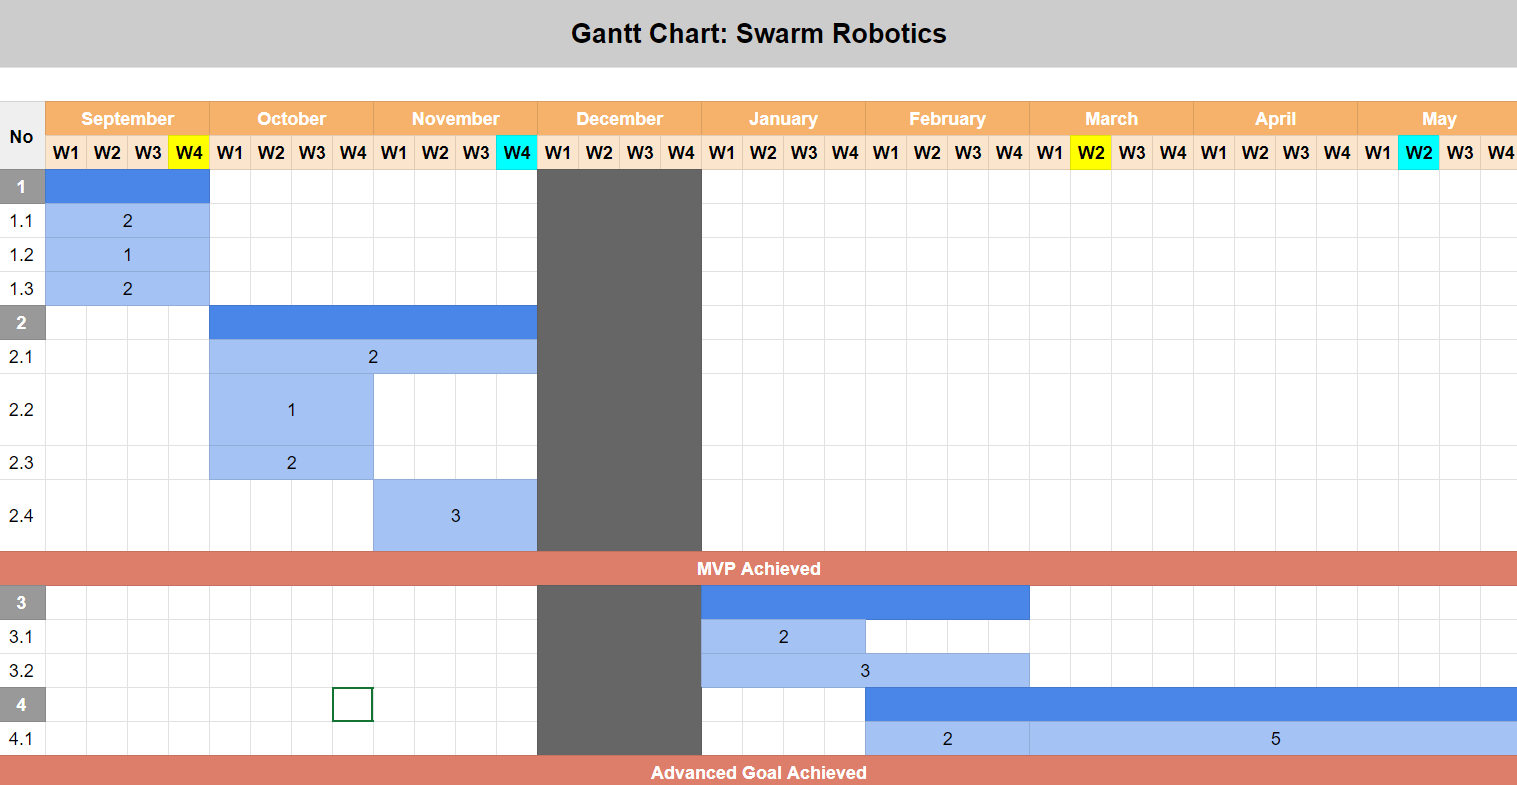
\includegraphics[width=1\linewidth]{assets/images/timeline/gantt_chart.png}
    \caption{Gantt Chart}
    \label{fig:Project Gantt Chart}
\end{figure}

\begin{enumerate}
    \item Preparation for Hardware Implementation
    \begin{enumerate}[label=1.\arabic*]
        \item Communication in the swarm
        \item Simple Simultaneous Localization and Mapping (SLAM) in Simulation
        \item Coordinated Gripping and Formation
        \item Object detection
    \end{enumerate}
    \item Moving Towards a Complete Swarm
    \begin{enumerate}[label=2.\arabic*]
        \item Hardware
        \item Movement after Gripping
        \item Testing and Evaluation
    \end{enumerate}
\end{enumerate}


\chapter{Theory Backup}

\section{Omnidirectional Movement}
\paragraph*{}
In the field of mobile robots, omnidirectional wheels have an advantage of moving in 2 degrees, 3 degrees of freedom. In the x-y axis and yaw. It's a holonomic locomotion unlike non-holonomic such as ackerman or differential drive. 90deg dual row would be the option of choice. The reason why we use omnidrive is because it can move in any direction without disengaging the object. Simple mechanism due to no linkage. Need a suspension.

\section{Waypoint Navigation}

\paragraph*{}
Repulsive Potential limitation is the local minima for the velocity at which the robot can travel, which can cause the roboto be stuck. This is where Rotational Fieldsand Random Fields come into play. By adding a rotational field around obstacles, the symmetry of the potential field is broken. As a result, the potential field will act as a guide for the robot to manoeuvre around groups of obstacles while avoiding local minima. However, this function can cause unstable oscillation during high speeds, narrow corridors, or sudden changes. 

\paragraph*{}
The Wavefront Planner applies the brushfire algorithm, starting from the goal and labelling the goal pixel as 2, then adding all zero neighbours. It continues iterating by updating distances for neighbouring cells and adding them to the list until all cells are processed. The final result provides a distance value for each cell, allowing the robot to follow a gradient descent by moving to the neighbour with the lowest distance value.

\section{Swarm Robotics Theory}

\paragraph*{}
Swarm Robotics is a robotics field that mimics the collective behaviour of natural swarms like ants, birds, and fish. The fundamental concept behind swarm robotics is to make use of multiple robots working together and carrying out tasks that would be difficult and inefficient for one single robot to handle. The four main principles of swarm robotics are self-organisation, distributed control, local interaction, and scalability. The principles are crucial for the robots to perform complex tasks by following simple individual instructions. Robots in a swarm are usually decentralised meaning that they operate on simple rules based on the local environment. This approach allows the swarm to be scaled easily as the number of robots increases\cite{beni1989swarm}.

\section{SLAM}

\paragraph*{}
Simultaneous Localisation and Mapping, also known as SLAM, is a crucial aspect of swarm robotics. SLAM is what allows each robot to navigate autonomously in an environment by constructing a map of said environment. While the map is being constructed, the robot is simultaneously tracking down their own position as well\cite{thrun2003probabilistic}. In our project, we will be using graph SLAM due to its accurate loop closure and global consistency. As a backup we can also use cartographer or SLAM toolbox, both of which are available as ROS2 packages.

\section{Object Detection and Computer Vision (CV)}

\paragraph*{}
LiDAR-camera fusion plays a vital role in object detection and pose estimation by combining the spatial accuracy and depth information from LiDAR with the detailed texture and appearance data provided by cameras. This dual-sensor approach overcomes the limitations of relying on a single sensor, offering improved accuracy and reliability in challenging and dynamic scenarios. Techniques such as Frustum PointNet utilise 2D image proposals to enhance 3D LiDAR point clouds, refining both object detection and pose estimation processes \cite{qi2018frustumpointnet}. Additionally, frameworks like MV3D and AVOD showcase the benefits of integrating LiDAR and camera data for real-time 3D object detection and pose estimation, ensuring precise localisation and interaction capabilities \cite{ku2018mv3d}, \cite{chen2017avod}. This methodology forms a robust foundation for the project, enabling accurate identification and positioning of objects, which is essential for practical applications in robotics.

\section{Multi-Robot Collaboration and Coordination}

\paragraph*{}
Dynamic Role assignment is going to be able to allow robots to adapt their behaviour based on the tasks at hand. This is important in tasks that require multiple and complex actions. By using the process of distributed decision-making, each robot evaluates its own capabilities and checks the status of other robots when making the decision to assume which role to take\cite{parker1998alliance}.

\section{Grasping and Object Manipulation in Robotics}

\paragraph*{}
In robotics, grasping and object manipulation are critical challenges that often require sophisticated algorithms for planning and controlling the end-effector, such as robotic grippers. In traditional robotic systems, grasp planning involves calculating the optimal points on an object to secure it, ensuring stable lifting and transport. This becomes particularly complex in cluttered or dynamic environments, where obstacles and unexpected changes may affect the robot’s ability to maintain a stable grasp. However, in swarm robotics, the collective behaviour of multiple robots can simplify this task. Instead of relying on a single robot to execute a complex grasp, multiple robots can collaborate in a more straightforward and effective manner. In our project, this is achieved using a sliding method for object manipulation, where one robot is responsible for pushing the object while the others stabilise it. This coordinated formation approach reduces the need for precise, complex grasp.


\chapter{Project Outcome}

Assuming we are able to reach our goal by overcoming expected and unexpected challenges. 

\paragraph*{}
\textbf{Stage 1: Collaborative Localization and Mapping Using GRAPH SLAM} \\
In the first stage, three robots are randomly placed within a room containing furniture and three distinct target objects. Each robot will independently scan the environment using LiDAR and Graph Simultaneous Localization and Mapping (Graph SLAM) to determine its own position, identify the relative positions of other robots, and collaboratively create a shared map of the room. This process continues until the entire space is mapped. The use of Graph SLAM is advantageous due to its ability to accurately represent and optimize large-scale environments by solving the graph of poses and constraints efficiently, which ensures consistent mapping even in complex environments. Though it requires more expensive sensors like LiDAR, this is offset by improved localization accuracy. This stage will be conducted at the ISE Lab.

\begin{figure}
    \centering
    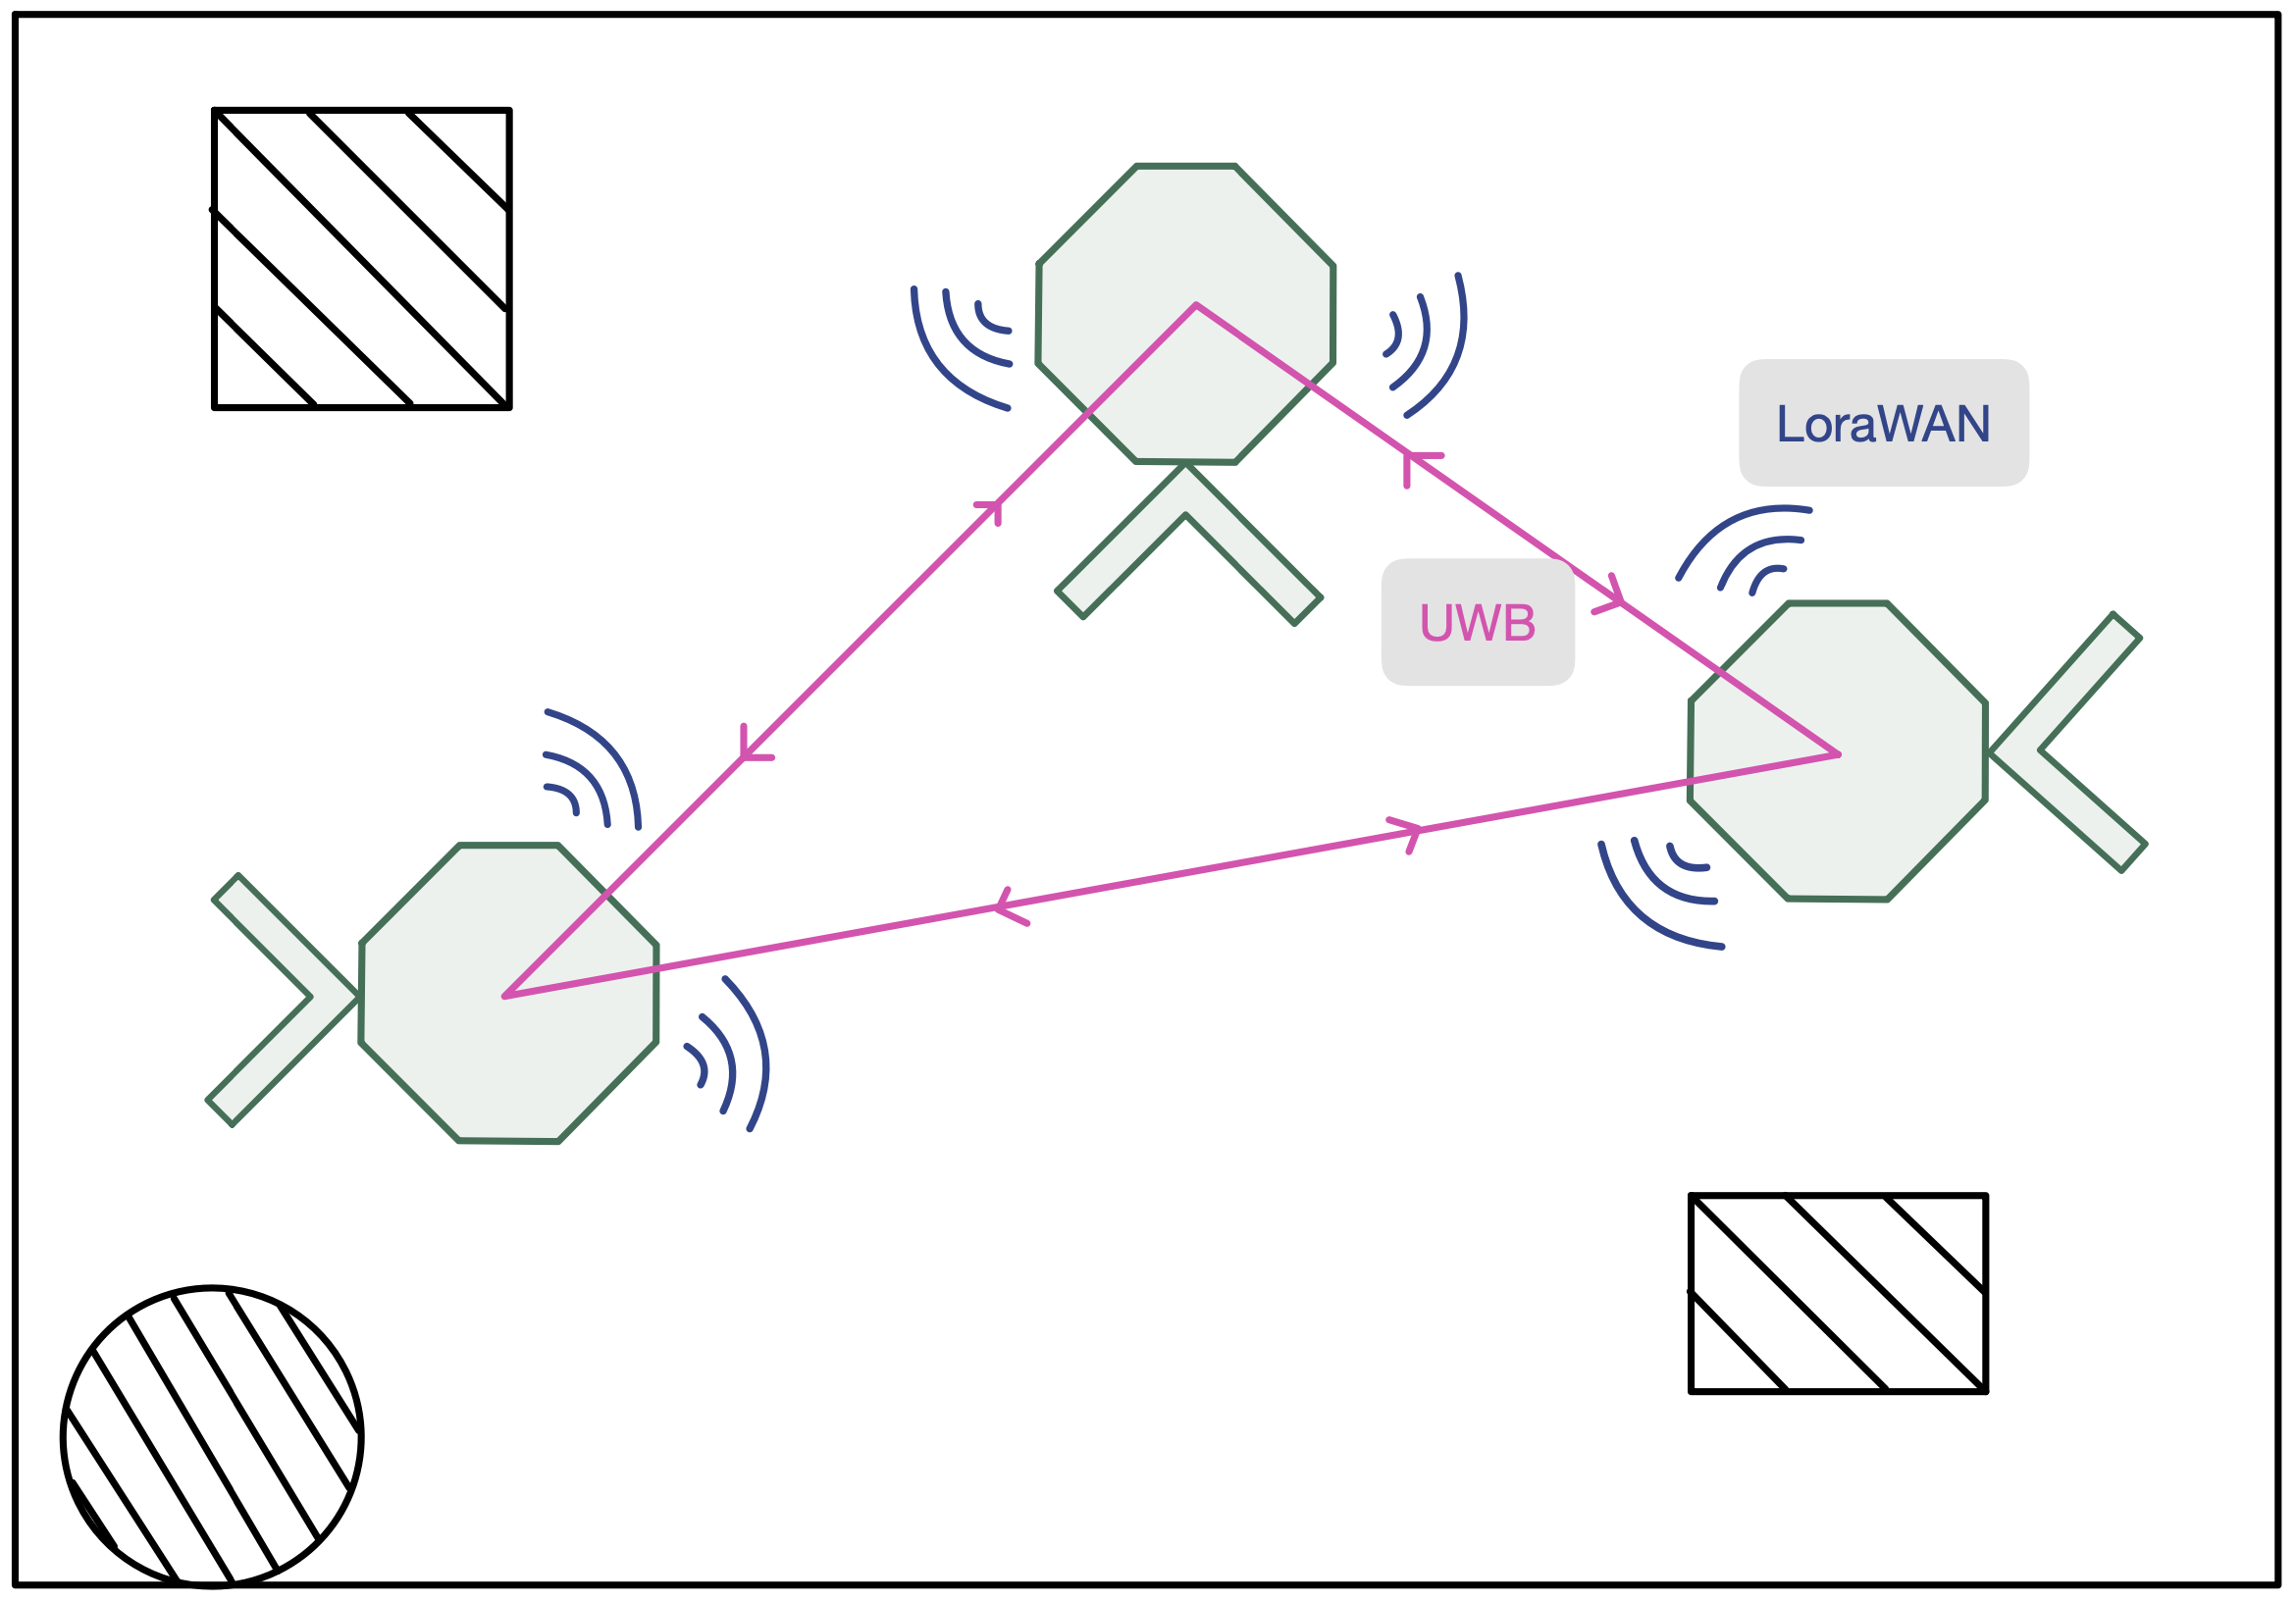
\includegraphics[width=0.5\linewidth]{assets/images/project_outcome/stage_1.png}
    \caption{Stage 1: 3 swarm robots(Green) localising and communicating with each other using WiFi. the black objects are obstruction}
    \label{fig:phase1}
\end{figure}

\paragraph*{}
\textbf{Stage 2: Object Detection and Consensus for Identification} \\
After localization is complete, the swarm enters a standby state. When a named object is selected from the model database, the robots will collaborate to search for and identify the object. Upon locating it, the robot communicates the object’s position to the rest of the swarm. A consensus mechanism ensures that over 50\% of the robots agree that the correct object has been identified before any action is taken. The object, for testing purposes, is a static, slid-able geometric shape, such as a cube. The robots utilise RGB-D cameras for dynamic object detection, ensuring that movable items like pets or furniture are not unintentionally displaced. The depth data from the cameras enhances the robots’ 3D mapping capabilities and provides a cost-effective solution for object recognition.

\begin{figure}
    \centering
    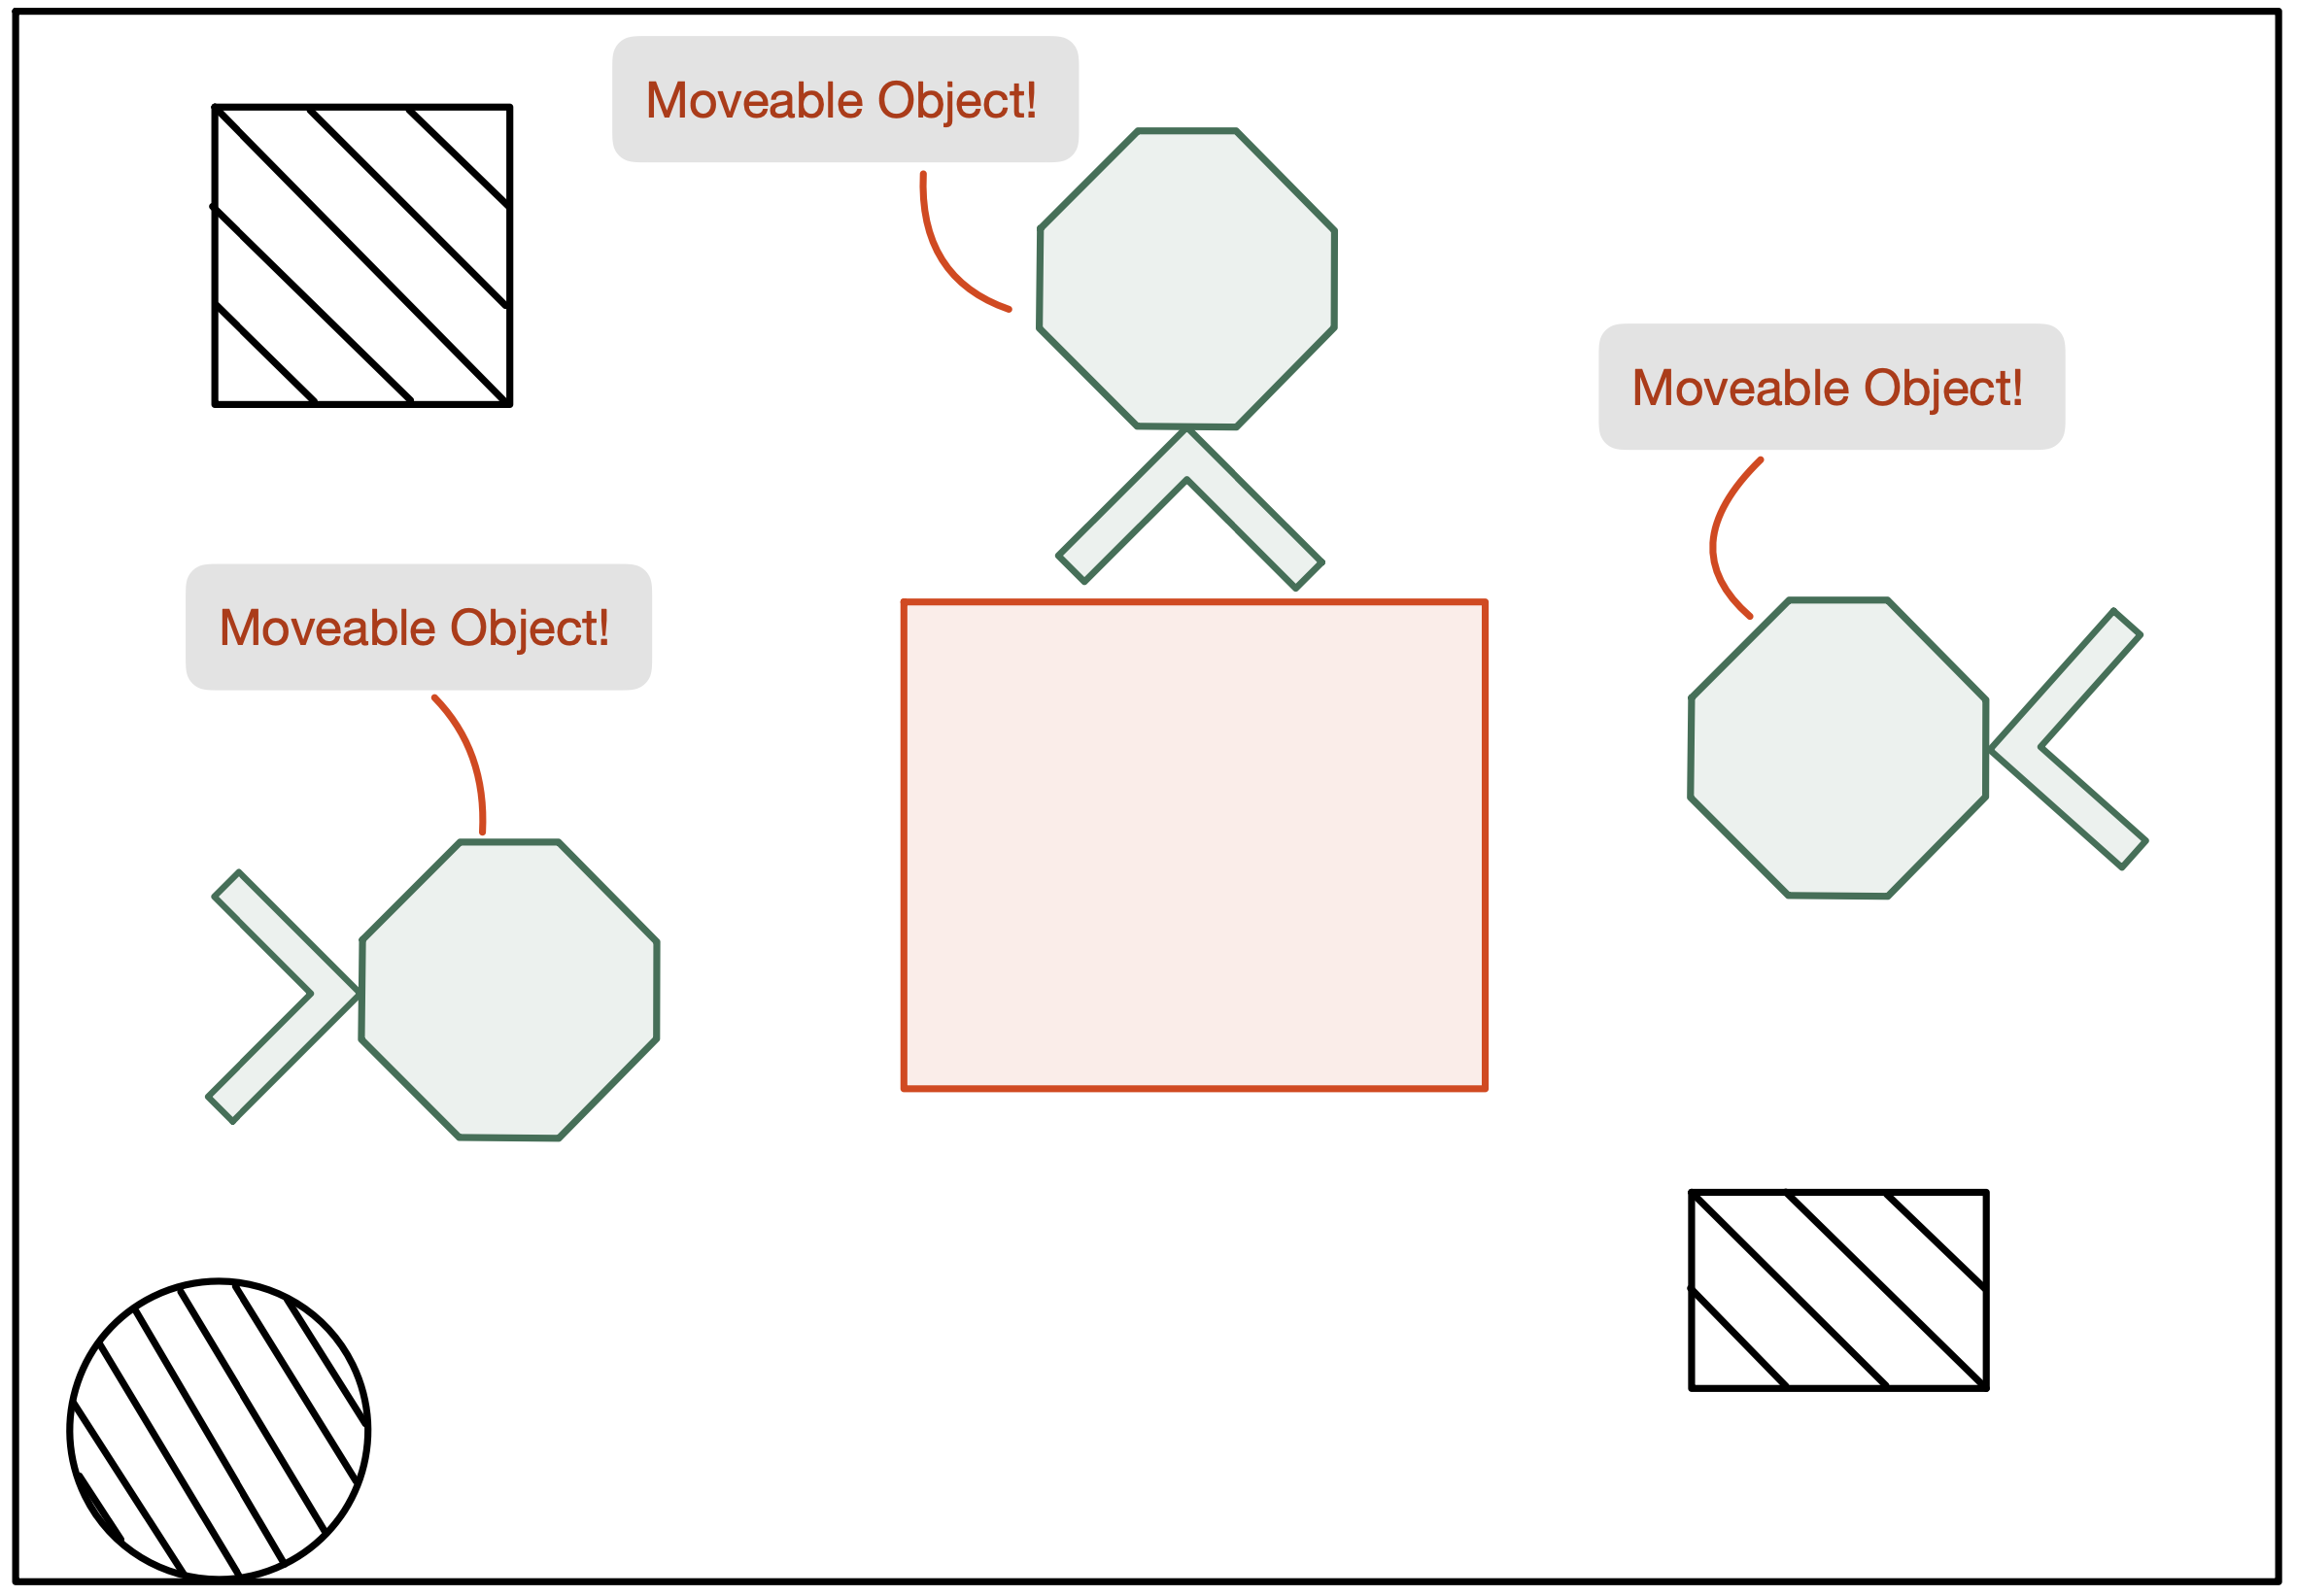
\includegraphics[width=0.5\linewidth]{assets/images/project_outcome/stage_2.png}
    \caption{Stage 2: A Red Object placed in the localised map, the robots detects the object using 2D/3D computer vision}
    \label{fig:phase2}
\end{figure}

\paragraph*{}
\textbf{Stage 3: Coordinated Object Movement} \\
Once consensus on the target object is reached, the robots will move towards it. Two robots, named Alpha and Beta, are assigned to secure the object along the X and Y axes at diagonal corners. A third robot, Gamma, provides the necessary force to push the object along a straight line toward its destination. The assignment of these roles is dynamic, with Alpha, Beta, and Gamma selected based on proximity to the object and destination. Alpha and Beta are assigned based on proximity to the object’s corners, while Gamma is the robot closest to the straight line between the object and destination. This method is both efficient and flexible, as role assignment occurs in real time, ensuring minimal delay. The destination is selected either by choosing the nearest edge of the object or by providing specific coordinates using the SLAM-generated map, allowing future integration with advanced interfaces like drag-and-drop UI.

\begin{figure}
    \centering
    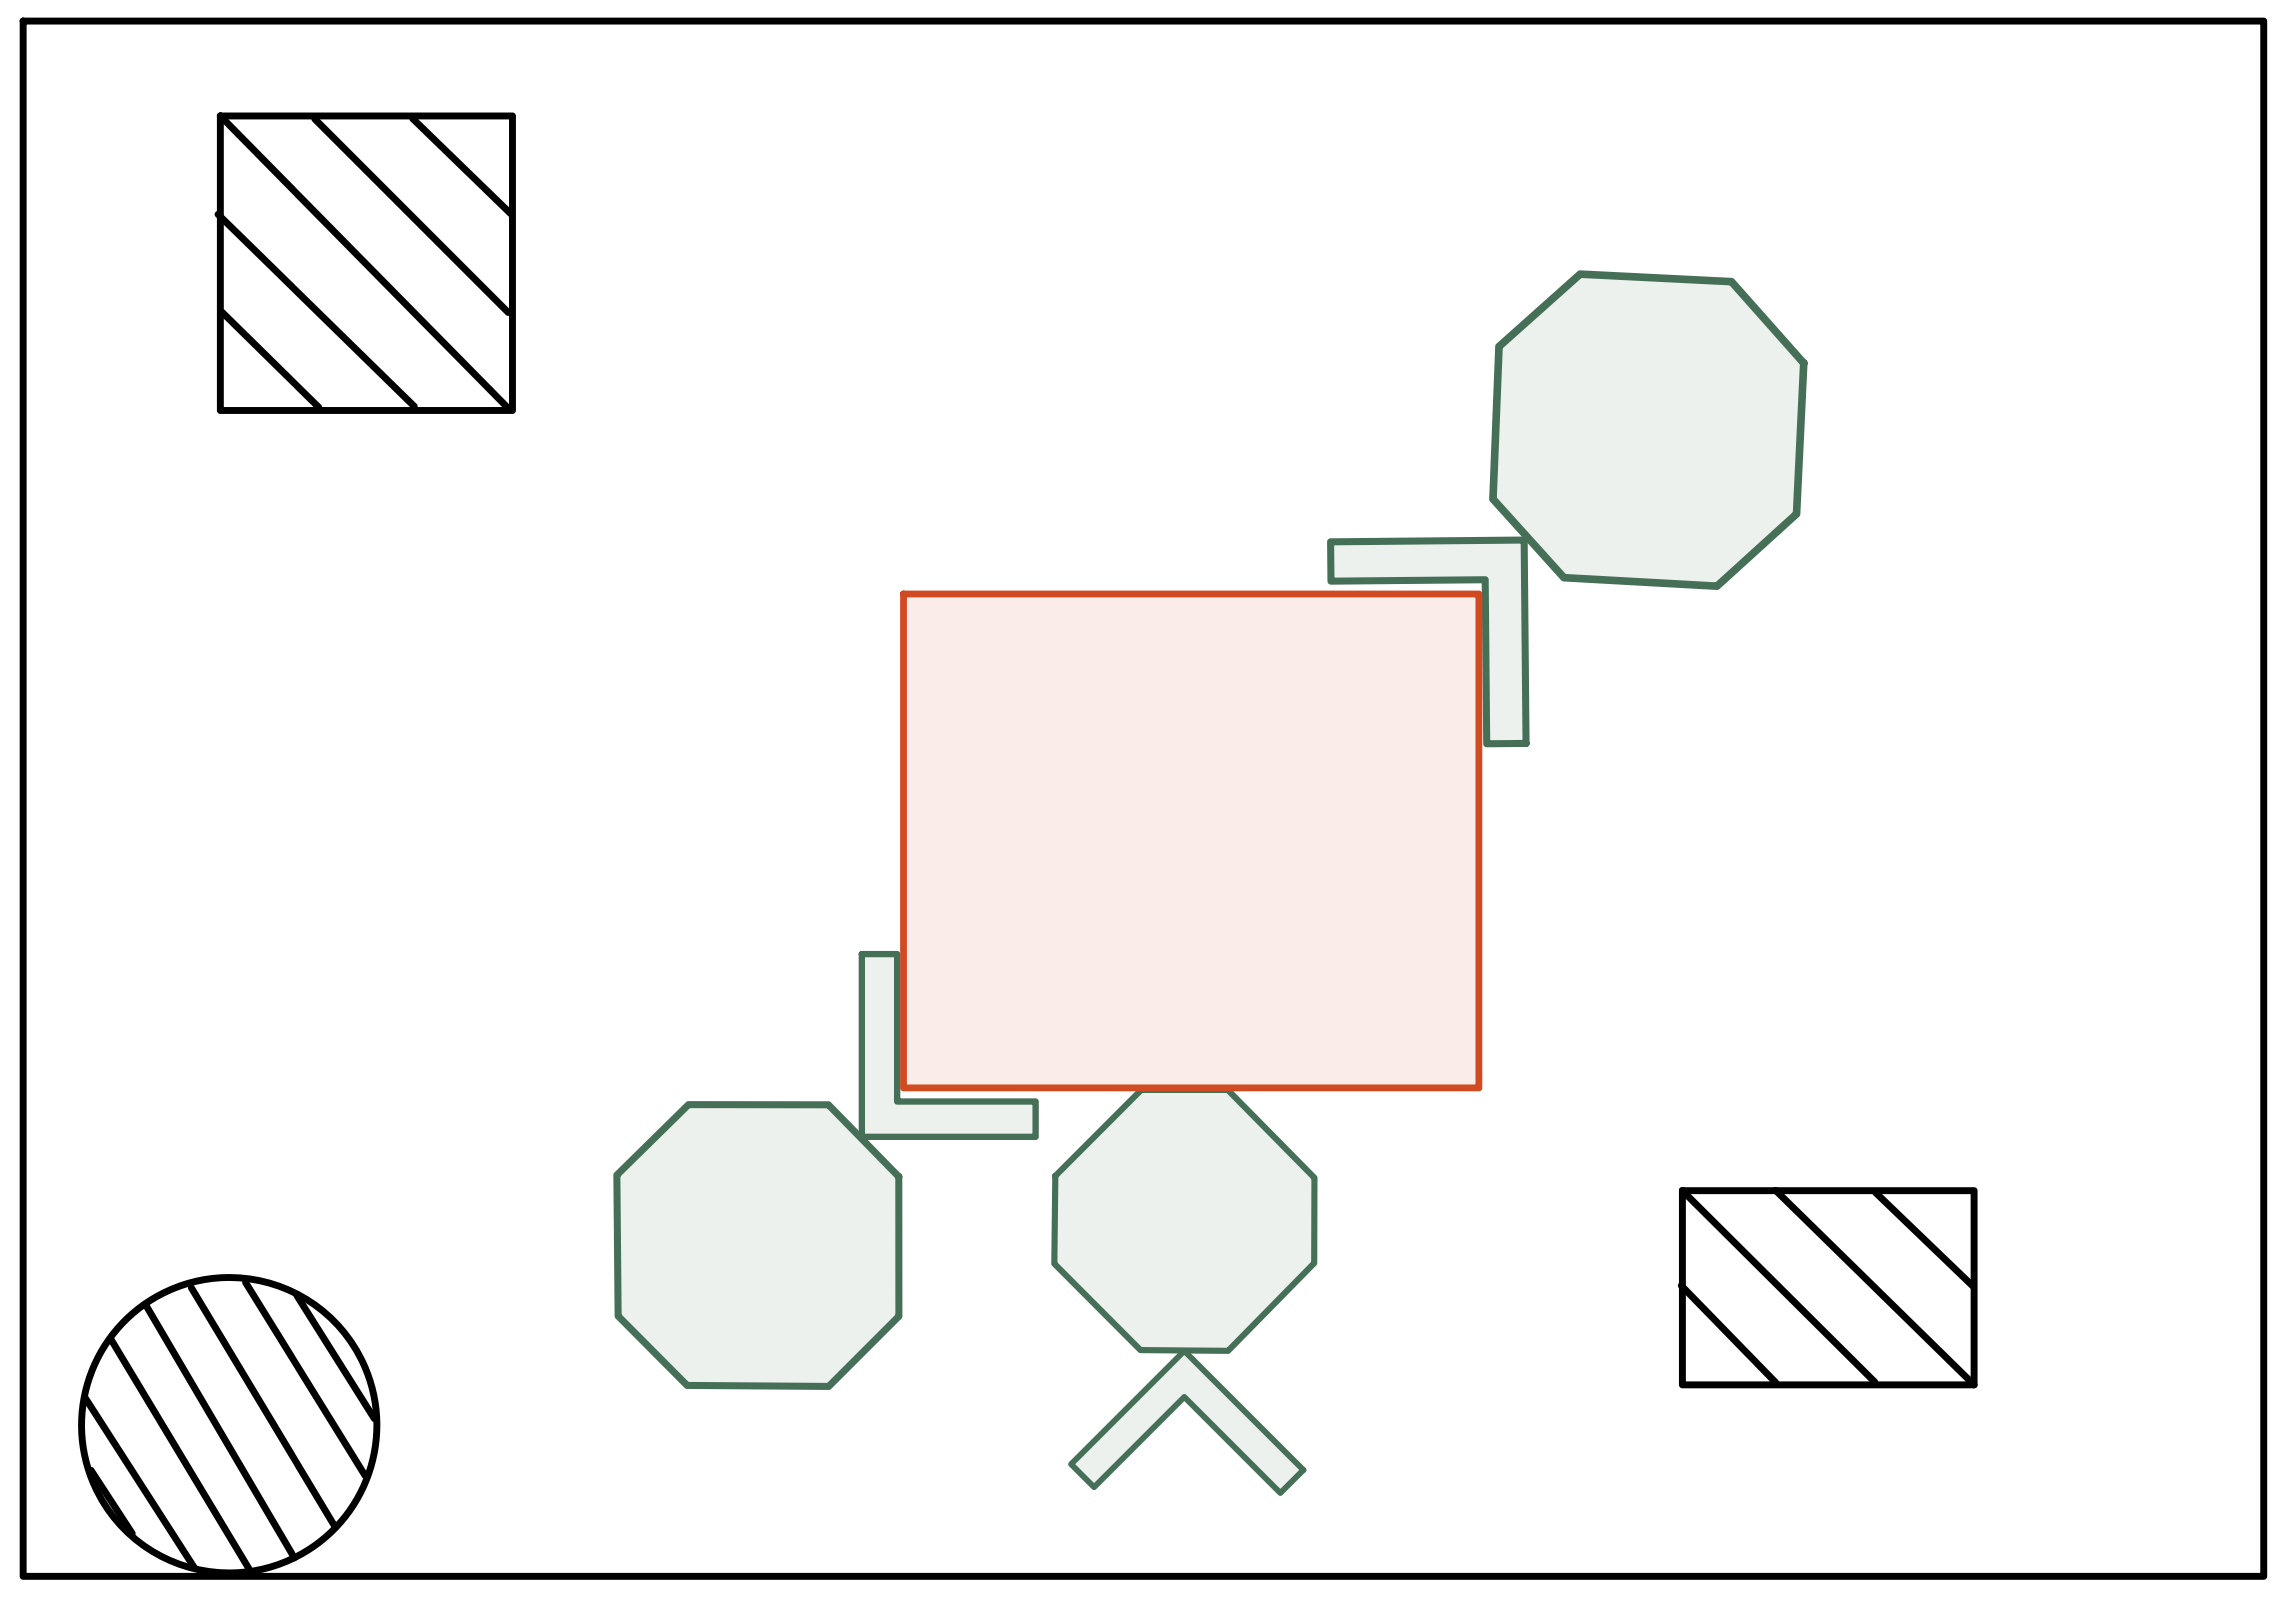
\includegraphics[width=0.5\linewidth]{assets/images/project_outcome/stage_3.png}
    \caption{Stage 3: The swarm moves and grip the object and ensure the object is securely in place}
    \label{fig:phase3}
\end{figure}

\paragraph*{}
\textbf{Stage 4: Object Movement and Environmental Constraints} \\
In the final stage, the robots push the object to the selected destination. To facilitate this, the object must have sufficiently low friction to allow sliding across the floor, as the team has chosen to restrict the object’s motion to two dimensions. The sliding method minimises potential challenges related to lifting or gripping the object

\begin{figure}
    \centering
    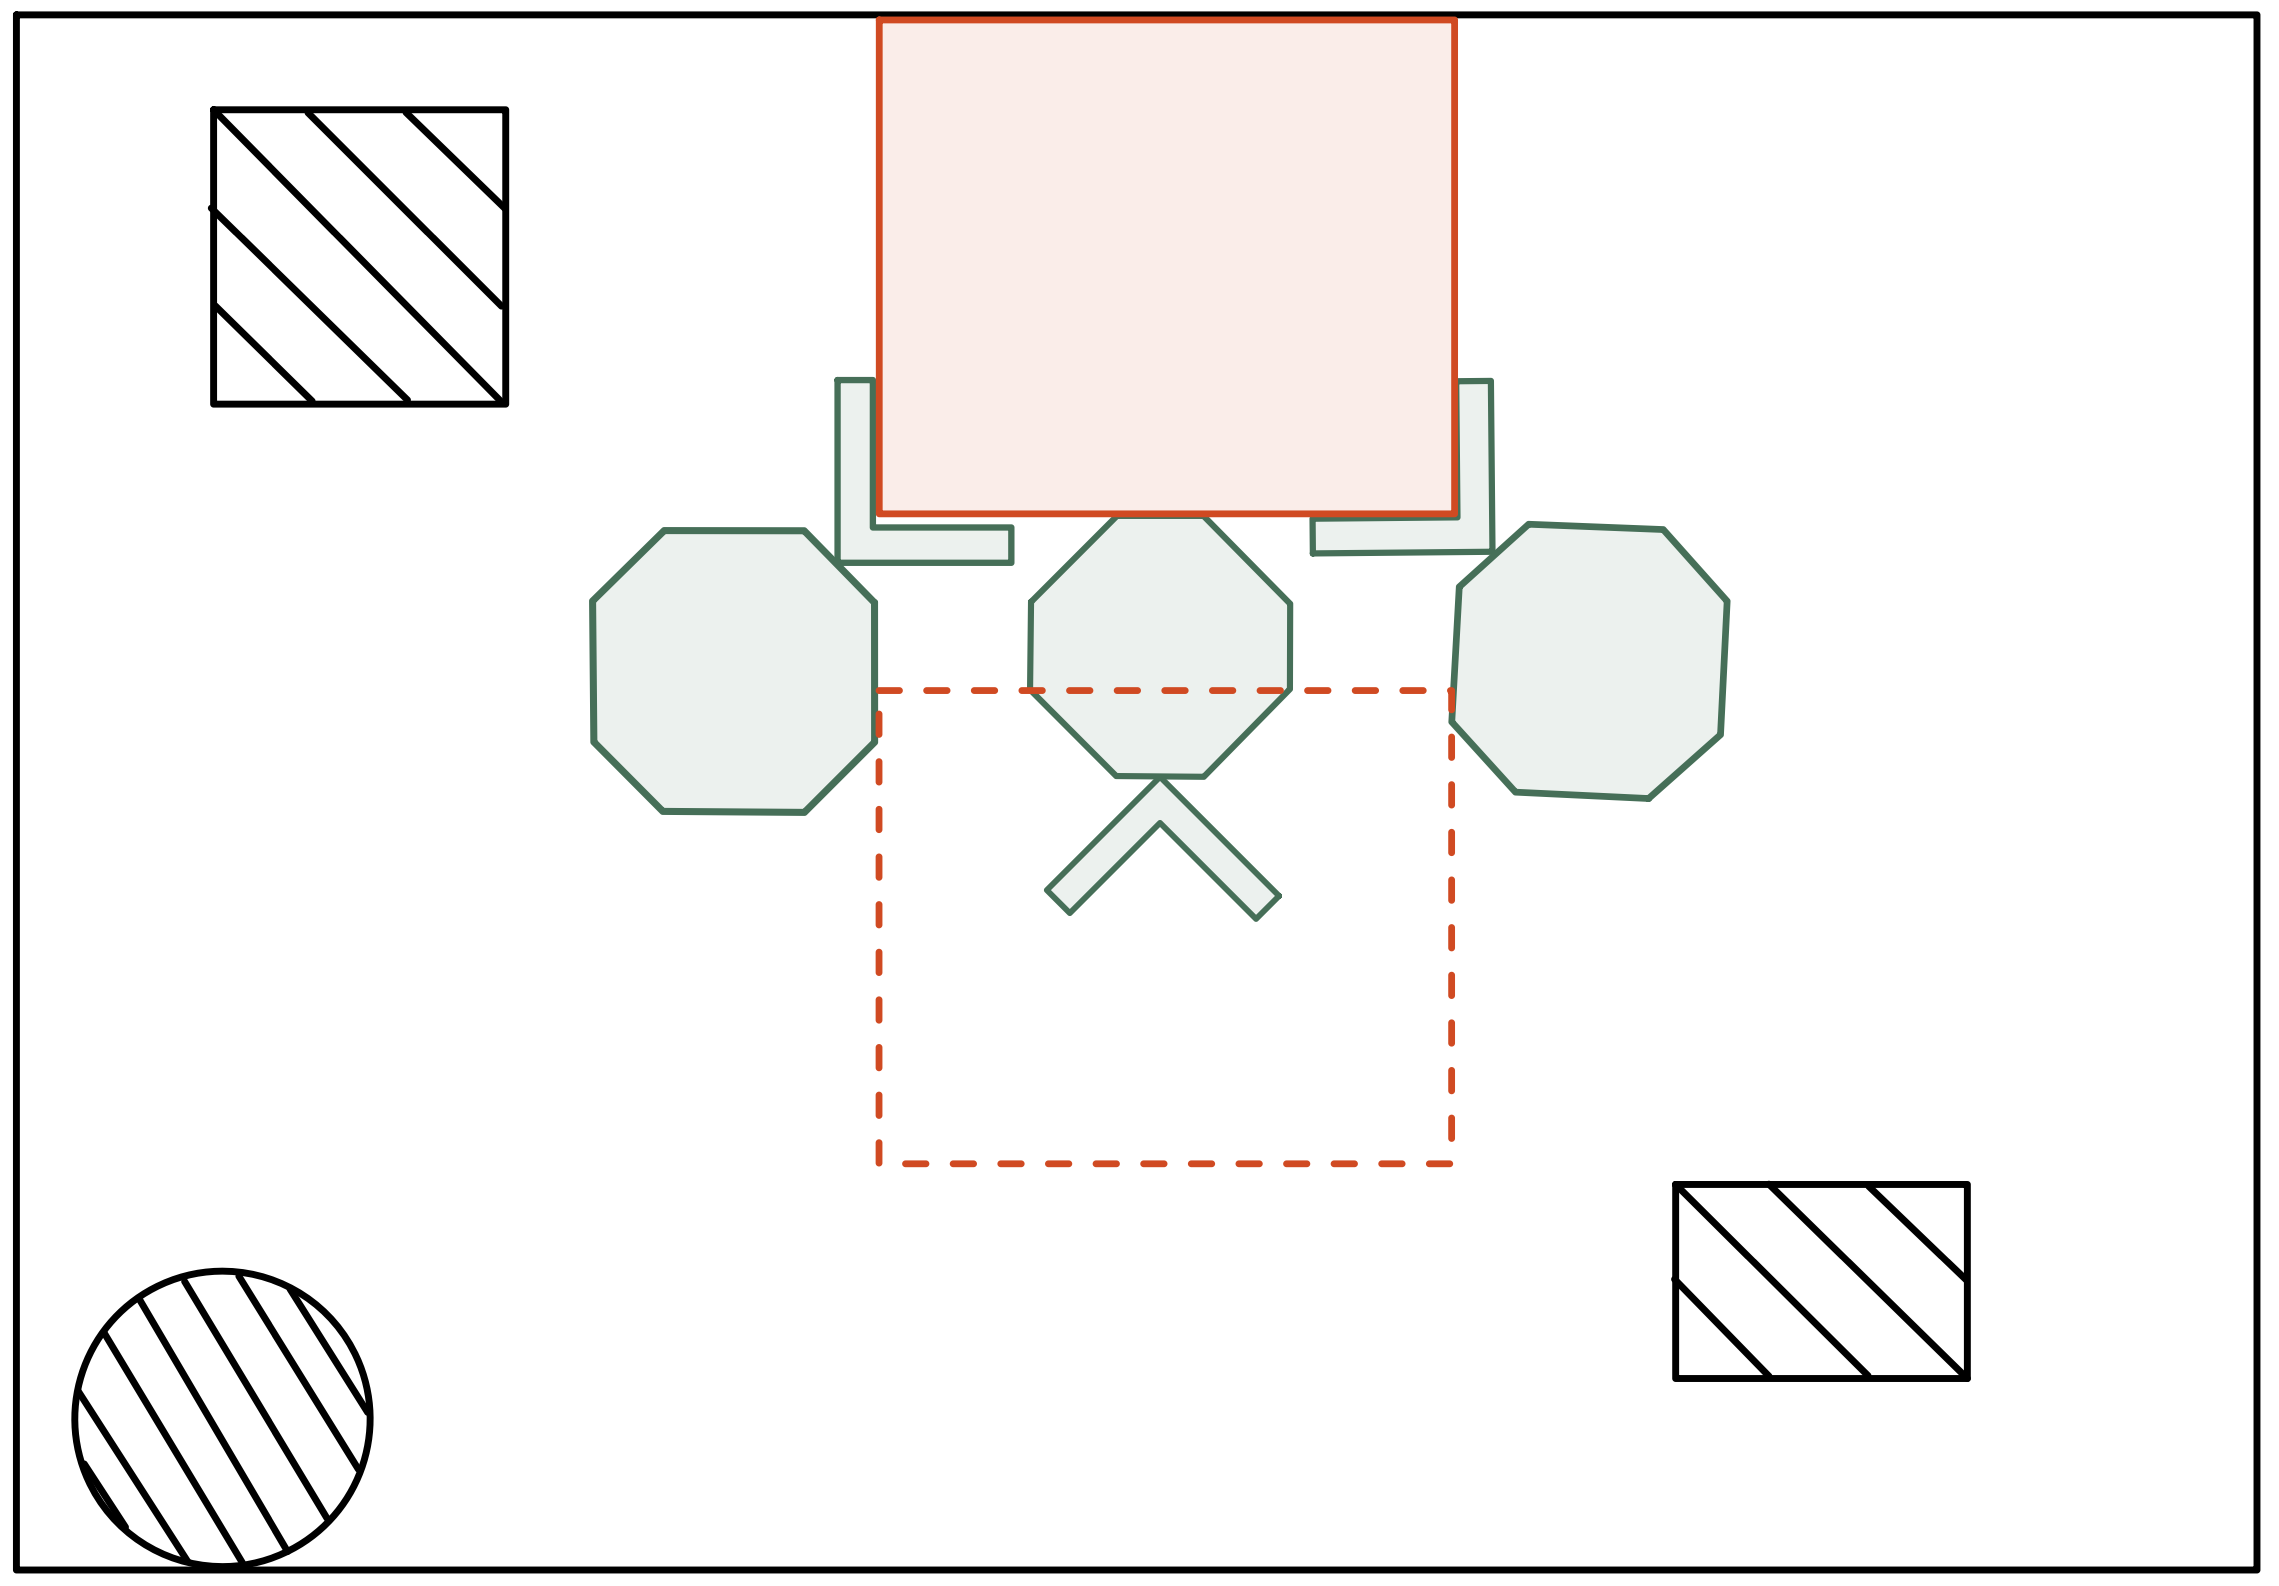
\includegraphics[width=0.5\linewidth]{assets/images/project_outcome/stage_4.png}
    \caption{Stage 4: The swarms then move the robot to the designated area and adjust the position of the robot dynamically}
    \label{fig:phase4}
\end{figure}


\chapter{Summary and Benefits to Real Industry}

\paragraph*{}
It’s becoming increasingly inevitable that robots will take over a significant portion of the workforce in the near future, especially for repetitive and monotonous tasks. As industries like warehousing, manufacturing, and even domestic environments integrate more robots, the ability for multiple robots to work together in the same space becomes critical. This is where swarm robotics comes into play. In such systems, robots must be able to communicate effectively to avoid collisions, coordinate task allocation, and share progress, ensuring smooth and efficient workflows. This project is a step toward achieving that goal by advancing decentralised, collective robotic behaviour.

\paragraph*{}
A key feature of this project is the decentralised communication system, where robots can interact with one another without needing a host computer or central control. This makes the system incredibly flexible and easy to deploy in various settings—whether in the field or at fixed locations like warehouses or homes. The decentralised nature allows for a plug-and-play style of operation, eliminating the need for complex initial setups. The mesh communication system also provides resilience, as the robots can continue working even if one or more units experience failure, ensuring task completion. This makes the system well-suited not just for static environments but also for dynamic, outdoor applications where flexibility is key.

\paragraph*{}
The benefits extend across various industries, from cleaning and tidying in commercial or domestic spaces (homes, offices, retail) to more complex environments like schools or factories where multiple robots operate together. The technology’s adaptability and resilience make it applicable in any scenario where more than one or two robots are required to collaborate, making it a valuable solution for the future of automation.


\chapter{Project Contribution per Student}

\paragraph*{}
In the first phase, the project tasks are divided among the group members to ensure a focused effort on simulating the fundamental components. Two group members will concentrate on developing the communication aspect, ensuring that the robots can coordinate and communicate effectively within the swarm. Simultaneously, one member will focus on object detection using computer vision techniques, while another two members tackle the basic implementation of SLAM (Simultaneous Localization and Mapping). This phase is scheduled to span from October to early November.

\paragraph*{}
Moving into the second phase, which runs from early November to early December, the project transitions to integrating hardware and enhancing SLAM functionalities. Initially, all group members will collaborate on incorporating simple movement into the hardware, ensuring a robust foundation for the next tasks. One group member will then test the SLAM implementation in two different environments to verify its effectiveness. Concurrently, two members will work on improving SLAM by developing a more advanced version, such as C-SLAM. After completing these tasks, the dedicated SLAM team, composed of three members, will integrate the individual modules from the first phase into a cohesive simulation, aiming to achieve a Minimum Viable Prototype by the semester's end.

\paragraph*{}
In the third phase, from January to early March of the second semester, the focus shifts to more advanced capabilities, including gripping mechanisms and coordinated movement. Two group members will work on the coordinated gripping task, preparing the static gripper for future sliding movements. Meanwhile, another three members will develop strategies for robot formation, ensuring that the robots can move together seamlessly after gripping objects.

\paragraph*{}
Finally, the fourth phase, starting in March and extending to early May, involves putting all the functional simulation components together with the actual robotic hardware. During this period, all group members will collaborate intensively to integrate these components, ensuring they work together smoothly in the real world.


\bibliographystyle{IEEEtran}
\bibliography{biblio}

\end{document} 